\documentclass[12pt]{ctexart}
\usepackage{amsmath} % 导入数学公式宏包
% 引入必要的宏包
\usepackage{amsthm}
\numberwithin{equation}{section} % 按 section 区分方程的编号
\newtheorem{theorem}{定理}[section]
\usepackage{lipsum}
\usepackage{multicol}
\usepackage[a4paper, margin=1in]{geometry}
\usepackage{xeCJK}
\usepackage{indentfirst}
\usepackage{setspace}
\usepackage{titlesec}
\usepackage{natbib}
\usepackage{fancyhdr}
\usepackage{unicode-math}
\usepackage{graphicx}
\usepackage{unicode-math} % 导入unicode-math宏包

% 设置数学字体
\setmathfont{Segoe UI Symbol}

% 设置页面格式和页眉页脚
\pagestyle{fancy}
\fancyhf{}
\fancyhead[R]{\thepage} % 页眉右侧显示页码
\fancyhead[L]{\textit{\small 计算物理}} % 页眉左侧显示标题
\renewcommand{\headrulewidth}{0pt} % 设置页眉分隔线宽度为0

\title{谱方法及其应用}
\author{李先宝 \and 林子熙 \and 刘子宁 \and 陈睿 \and 段尚福 \and 郑文龙}
\date{}

% 文档开始
\begin{document}

\maketitle
\begin{abstract}
    本论文详细介绍了我们六人团队在计算物理领域的合作成果,特别聚焦于谱方法(Spectral Methods)在求解偏微分方程中的应用。谱方法以其在高维空间中的高效性和精确性而著称,我们通过本项目深入探讨了该方法的理论基础、数值实现及其在物理问题中的应用。

在理论探讨中,我们首先回顾了正交多项式的基础,阐明了它们在构建谱方法中的关键作用。我们进一步分析了高斯-勒让德积分法,这是一种利用正交多项式节点进行数值积分的技术,它为谱方法提供了精确的积分工具。此外,我们详细讨论了Galerkin方法和配点法(Collocation),这两种技术在谱方法中用于构建近似解和处理边界条件。

在应用层面,我们选择了n维超球面的积分问题作为研究案例,展示了谱方法如何将复杂的多维积分问题转化为易于求解的代数问题。我们还探讨了谱方法在电磁学和量子力学中的应用,包括使用Galerkin方法求解薛定谔方程和利用配点法处理边值问题。

项目实践中,四位团队成员负责理论分析和算法编程,通过数值实验验证了谱方法的有效性。一位成员负责制作PPT,清晰地展示了我们的研究成果。另一位成员负责撰写本论文,全面记录了我们的研究方法、过程和结论。

通过本项目,我们不仅加深了对谱方法的理解,而且提升了团队协作和编程技能。我们的研究结果证明了谱方法在解决复杂物理问题中的潜力,为计算物理及相关领域的研究提供了新的视角和工具
\end{abstract}
\newpage
\tableofcontents
\newpage
\section{引言}
在计算物理的研究中,谱方法因其在处理高维问题时的高效性和精确性而受到广泛关注。该方法通过将连续的物理问题转化为离散的代数问题,极大地简化了问题的求解过程。正交多项式作为谱方法的核心,提供了一组在特定权重函数下正交的基函数,这为问题的近似求解提供了便利。

本研究首先系统地介绍了谱方法的理论基础,包括正交多项式的构造、性质以及高斯-勒让德积分法的应用。我们特别强调了Galerkin方法和配点法在谱方法中的重要性。Galerkin方法通过最小化残差的能量范数来求解问题,而配点法则通过在一组选定的点上满足方程来构造近似解。

在应用研究中,我们选择了n维超球面的积分问题作为谱方法应用的案例。通过变量替换和Jacobian行列式的计算,我们展示了如何将问题转化为谱方法可以高效求解的形式。此外,我们还探讨了谱方法在电磁学中的电势计算和量子力学中的薛定谔方程求解中的应用。

通过本项目,我们不仅在理论上取得了突破,而且在编程实现、演示制作和论文撰写等方面也取得了显著成果。我们的研究结果展示了谱方法在解决复杂物理问题中的潜力,并为未来的研究提供了新的思路和工具。
\section{正交多项式和高斯型积分方法及其在n维超球的积分求解中的应用 }
\subsection{正交多项式简介}
\subsubsection{函数正交的定义}
记区间$[a,b]$中所有的连续函数为$C[a,b]$ ,设$f(x),g(x)\in C[a,b]$ , $\omega(x)$是$[a,b]$上的权函
数,若:
\begin{equation}
    (f,g)_\omega=\int_a^b\omega(x)f(x)g(x)dx=0
\end{equation}
则称$f(x)$与$g(x)$在$[a,b]$上 带权$\omega(x)$正交。
\subsubsection{正交多项式的定义}
正交多项式的定义是正交函数族的一个特殊情况,即正交函数族中的函数全部为多项式的情况。

设$\{p_n(x)\}$是首项系数$k_n\neq0$的$n$次多项式,$\omega(x)$是定义在$[a,b]$上的权函数,若:
\begin{equation}
    (p_i,p_j)_\omega = \int_a^b \omega(x) p_i(x) p_j(x) \mathrm{d}x = 
    \begin{cases}
        0, & i \neq j, \\
        A_i > 0, & i = j
    \end{cases} \quad (j,k=0,1,\cdots)
\end{equation}
则称多项式序列$\{p_n(x)\}$在$[a,b]$上带权$\omega(x)$正交,并称$p_n(x)$是$[a,b]$上带权
$\omega(x)$的$n$次正交多项式。

可以由线性无关的一组基$\{1,x,x^2,\ldots,x^n,\ldots\}$按Schemite正交化过程构造正交化多项式,

其中
$p_0(x)=k_0\text{ ,}$
\begin{equation}
    p_n(x)=x^n-\sum_{k=0}^{n-1}\frac{(x^n,p_k)_\omega}{\|p_k\|_\omega^2}p_k(x),\quad k=1,2,\ldots 
\end{equation}
\subsubsection{正交多项式的递推关系}
设 $\{p_n\}$ 是定义在$[a,b]$上的正交多项式序列,其首项系数$k_{n}\neq 0.$ 
那么我们有
\begin{equation}
    p_{n+1}=(a_nx-b_n)p_n-c_np_{n-1},\quad n\geq0,
    \label{eq:正交多项式的递推关系}
\end{equation}
其中 $p_{- 1}: = 0$, $p_{0}= k_{0}$ 

以及
\begin{equation}
    \begin{cases}
        \begin{aligned}
            a_{n} &= \frac{k_{n+1}}{k_{n}} \\
            b_{n} &= \frac{k_{n+1}}{k_{n}} \frac{(xp_{n}, p_{n})_\omega}{\|p_{n}\|_{\omega}^{2}} \\
            c_n &= \frac{k_{n-1}k_{n+1}}{k_n^2} \frac{\|p_n\|_{\omega}^2}{\|p_{n-1}\|_{\omega}^2}
        \end{aligned}
        \label{特征值方法的矩阵元}
    \end{cases}
\end{equation}
\subsubsection{正交多项式的零点}
正交多项式的零点也具有良好的性质,其零点是实的,且都分布在$[a,b]$上(具体证明见相关专著)。
下面我们给出计算正交多项式零点的方法即\textbf{特征值方法}。

\begin{theorem}
$n+1$次正交多项式$p_{n+1}(x)$的零点是以下对称矩阵的特征值

\begin{equation}
    A_{n+1}=\begin{bmatrix}\alpha_0&\beta_1\\\beta_1&\alpha_1&\beta_2\\&\ddots&\ddots&\ddots\\&&\beta_{n-1}&\alpha_{n-1}&\beta_n\\&&&\beta_n&\alpha_n\end{bmatrix},
\label{eq:零点矩阵}
\end{equation}
    
这里
$$\alpha_j=\frac{b_j}{a_j},\quad j\ge0;\quad\beta_j=\frac{1}{a_{j-1}}\sqrt{\frac{a_{j-1}c_j}{a_j}},\quad j\ge1,$$



而 $\{ a_{j}, b_{j}, c_{j}\}$ 是由(\ref{特征值方法的矩阵元})式定义出来的系数。
\label{theorem:零点矩阵}
\end{theorem}


























\subsection{正交多项式与高斯型积分公式}
我们现在讨论正交多项式与高斯型积分公式之间的关系。高斯型求积的机制是通过选择最佳节点来寻求对积分的最佳数值逼近。它属于数值求积的家族之一。
\begin{equation}
    \int^b_af(x)\omega(x)dx=\sum^N_{i=0}f(x_j)\omega_j+E_N[f]
    \label{eq:高斯求积公式}
\end{equation}
这里 $\{x_j,\omega_j\}_{j=0}^N$ 是求积公式的节点和权重, $E_N[f]$求积公式的误差。
\begin{equation}
    E_N[f]=\frac{1}{(N+1)!}\int_a^bf^{(N+1)}(\xi(x))\prod_{i=0}^N(x-x_i)dx,
\end{equation}

这里,$\xi(x) \in [a,b]$

如果 $E_N[f]\equiv0$, 我们称求积公式(\ref{eq:高斯求积公式})对于 
$𝑓$是精确的。


 



现在我们不加证明地介绍一些有用的定理

\begin{theorem}
    定义在$[a,b]$上的正交多项式  $p_{N+1}$  有零点$\{x_j\}_{j=0}^N$ 。则存在唯一一组积分权重使得,
\begin{equation}
\int_a^bp(x)\boldsymbol{\omega}(x)dx=\sum_{i=0}^Np(x_j)\boldsymbol{\omega}_j,\quad\forall p\in P_{2N+1},
\end{equation}

其中,该$\{\omega_j\}_{j=0}^N$ 可由下式定义:
\begin{equation}
    \omega_j=\int_a^bh_j(x)\omega(x)dx,\quad0\leq j\leq N.
\label{eq:积分权重}
\end{equation}

$ h_j(x)=\prod_{i=0;i\neq j}^N\frac{x-x_i}{x_j-x_i},\quad0\leq j\leq N$,即拉格朗日基函数
\label{theorem:多项式积分定理}
\end{theorem}
\begin{theorem}
    

设
\begin{equation}
    \mathbf{Q}(x_j)=\begin{pmatrix}Q_0(x_j),Q_1(x_j),\ldots,Q_N(x_j)\end{pmatrix}^T
\end{equation} 
为与$x_j$对应的矩阵(\ref{eq:零点矩阵})式的正交归一特征向量。

 即
 \begin{equation}
    A_{N+1}\mathbf{Q}(x_j)=x_j\mathbf{Q}(x_j)\quad \text{并且}\quad\mathbf{Q}(x_j)^T\mathbf{Q}(x_j)=1.
\end{equation}
    
那么权重$\{\omega_j\}_{j=0}^{N}$ 可以通过特征向量的第一个元素计算得出:
\begin{equation}
    \omega_j=\begin{bmatrix}Q_0(x_j)\end{bmatrix}^2\int_a^b\omega(x)dx,\quad0\leq j\leq N.
\end{equation}
\label{theorem:特征向量积分权重}
\end{theorem}
\textbf{
将正交多项式与高斯型积分公式结合起来:对于一个在$[a,b]$上的带权定积分,只需要知道它在特定点(正交多项式零点)上的函数值,就可以计算出带权积分的近似结果。这便使我们的积分求解精确便捷}
\subsection{超球问题}
\subsubsection{问题描述}
对于一个$n$维的平直空间,$n$维超球的表面满足$\sum ^n_{i=1}x_i^2=R^2$,

试求:该超球的体积$V_n(R)=\int_Vdv$。
\subsubsection{$n$维超球的换元公式}
\begin{enumerate}
    \item 令 $x_1 = r \cos \varphi_1 = rc_1$,则我们有
    \[
    x_2^2 + x_3^2 + \cdots + x_n^2 = (r \sin \varphi_1)^2 = (rs_1)^2.
    \]
    \item 整理后
    $$(\frac{x_2}{rs_1})^2+(\frac{x_3}{rs_1})^2+\cdots+(\frac{x_n}{rs_1})^2=1$$
   \item 继续令$\frac{x_2}{rs_1}=\cos\varphi_2=c_2$得$x_2=rs_1c_2$及
$$(\frac{x_3}{rs_1})^2+\cdots+(\frac{x_n}{rs_1})^2=s_2^2$$
   \item 如此反复下去即可得到我们的换元公式
   \begin{equation}
    \begin{aligned}
        \begin{cases}
            x_{1}=r\cos(\varphi_1), \\
            x_{2}=r\sin(\varphi_1)\cos(\varphi_2), \\
            x_{3}=r\sin(\varphi_1)\sin(\varphi_2)\cos(\varphi_3), \\
            ...\\
            x_{n-1}=r\sin(\varphi_1)\cdots\sin(\varphi_{n-2})\cos(\varphi_{n-1}), \\
            x_{n}=r\sin(\varphi_1)\cdots\sin(\varphi_{n-2})\sin(\varphi_{n-1}). 
       \end{cases}
     \end{aligned}   
   \end{equation}
   $r \in [0,R],\varphi_1,\cdots,\varphi_{n-2}\in[0,\pi)\text{ 以及 }\varphi_{n-1}\in[0,2\pi).$
\end{enumerate}
\subsubsection{Jaccobi行列式}
对应Jacobi矩阵行列式结果:
\begin{equation}
\begin{split}
    d^nv&=|det\frac{\partial(x_i)}{\partial(r,\varphi_j)}|drd\varphi_1\cdots d\varphi_{n-1}\\
    &=r^{n-1}sin^{n-2}(\varphi_1)\cdots sin(\varphi_{n-2})drd\varphi_1\cdots d\varphi_{n-1}
\end{split}
\end{equation}

于是我们要的求解形式转化为:
\begin{equation}
    V_{n}\left(R\right)=\int_{0}^{R}\int_{0}^{\pi}\cdots\int_{0}^{2\pi}r^{n-1}\sin^{n-2}(\varphi_1)\sin^{n-3}(\varphi_2)\cdots\sin(\varphi_{n-2})drd\varphi_1d\varphi_2\cdots d\varphi_{n-1}
\end{equation}

在这种换元下,积分变量相互独立,于是我们继续划分为三个子问题:
\begin{equation}
    \begin{aligned}
        \begin{cases}
        \int_0^R r^{n-1} dr \quad \text{\textcircled{1}}\\\\
        \prod\limits_{m=1}^{n-2} \int^\pi_0 \sin^m \theta \, d\theta \quad \text{\textcircled{2}} \\\\
        \int^{2\pi}_0 d\varphi \quad \text{\textcircled{3}}
    \end{cases}
 \end{aligned}
\end{equation}

\subsection{问题求解}
\subsubsection{雅可比多项式及雅可比-高斯型积分公式}
\textbf{定义}:在区间$(-1,1)$有权函数$\omega^{\alpha,\beta}(x) = (1-x)^\alpha(1+x)^\beta $,定义首项$J^{\alpha,\beta}_0(x)=1$经(\ref{eq:正交多项式的递推关系})式递推生成的多项式$\{J^{\alpha\beta}_n(x)\}$称为雅可比多项式,其中$\alpha》-1,\beta>-1$为多项式的两个参数

根据\textbf{定理}\ref{theorem:多项式积分定理},其对应的\textbf{雅可比-高斯型积分公式}如下:


\begin{equation}
    \int_{-1}^1p(x) \omega^{\alpha,\beta}(x)dx=\sum_{j=0}^Np(x_j)\omega_j,\quad\forall p\in P_{2N+1}
\label{eq:雅可比-高斯型积分公式}
\end{equation}


% \begin{equation}
%     \omega_j=\frac{G_N^{\alpha,\beta}}{J_N^{\alpha,\beta}(x_j)\alpha_xJ^{\alpha,\beta}_{N+1}(x_j)}
% \end{equation}
% \begin{equation}
%     G^{\alpha,\beta}_N=\frac{2^{\alpha+\beta}(2N+\alpha+\beta+2)\Gamma(N+\beta+1}{(n+1)!\Gamma(N+\alpha+\beta+2)}
% \end{equation}
% \begin{equation}
%     J_n^{\alpha,\beta}(x)=\frac{1}{n+\alpha+\beta}[(n+\beta)J_n^{\alpha,\beta-1}+(n+\alpha)J_n^{\alpha-1,\beta}(x)]
% \end{equation}
根据\textbf{定理}\ref{theorem:零点矩阵}和\textbf{定理}\ref{theorem:特征向量积分权重}:

% 雅可比多项式
$J_{N+1}^{\alpha,\beta}$
的零点$x_j$为以下三对角矩阵的特征值\\
% 补:(推论)高斯求积公式的最优横坐标,为对应相同区间的正交多项式的零点。\\
\begin{equation}
    A_{N+1}=
    \begin{bmatrix}
        a_0&\sqrt{b_1}&&\\
        \sqrt{b_1}&a_1&\ddots&\\
        &\sqrt{b_2}&\ddots&\sqrt{b_N}\\
        &&\sqrt{b_N}&a_N
    \end{bmatrix}
\end{equation}
其中:
\begin{equation*}
    a_j=\frac{\beta^2-\alpha^2}{(2j+\alpha+\beta)(2j+\alpha+\beta+2)}
\end{equation*}
\begin{equation*}
    b_j=\frac{4j(j+\alpha)(j+\beta)(j+\alpha+\beta)}{(2j+\alpha+\beta-1)(2j+\alpha+\beta)^2(2j+\alpha+\beta+1)}
\end{equation*}
(说明:由于雅可比多项式的参数$\alpha,\beta$容易与定理\ref{theorem:零点矩阵}中$\alpha,\beta$混淆,故在公式及说明上与定理\ref{theorem:零点矩阵}有所不同,请读者加以甄别)

而积分权重$\omega_j$与对应特征向量$ \mathbf{Q}(x_j)=\begin{pmatrix}Q_0(x_j),Q_1(x_j),\ldots,Q_N(x_j)\end{pmatrix}^T$的第一个元素有关
\begin{equation}
    \omega_j=\frac{2^{\alpha+\beta+1}\Gamma(\alpha+1)\Gamma(\beta+1)}{\Gamma(\alpha+\beta+2)}[Q_0(x_j)]^2
\end{equation}
\subsubsection{将一般积分转化为带权积分}
对于一般的$g(x)\in C[a,b]$,$\int_a^b g(x)$的求解通过选择适当的权函数可以转化为带权积分,而带权积分的求解利用上述定理可以迅速将误差缩小。

下面将给出一些示例:
\begin{itemize}
    \item  $I = \int_{-1}^{1} \sqrt{1-x^2} \, dx$

    这里考虑用带权积分来求解$I$,首先选取权函数为$\omega(x)=\omega^{1,1}(x)$
    
    则:
    $$I=\int_{-1}^{1} \omega^{1,1}(x)\, dx$$
    根据公式(\ref{eq:雅可比-高斯型积分公式}),知道这里的$p(x)=1$,通过在正交多项式零点上取值,就可以计算积分$I$的结果,并且很容易就可以实现$E_N(\sqrt{1-x^2})=0$

\end{itemize}

当然对于任意的积分都可以令$\omega(x)=1$,这样可以自动考虑带权结果。但必须强调的是:权函数的选取具有重要意义,对于一些看似不能精确求解或者有效求解(指收敛速度很快)的积分,通过选取适当的权函数,可以大大提高积分精度和收敛速度。

所以对于超球问题中的三个积分,我们也需要通过选择适当的权函数,和精心的设计,来实现超球问题中的积分求解。

\subsubsection{具体设计}
  \begin{itemize}
    \item 对于积分\textcircled{1}\begin{equation}
        I_1=\int^R_0 r^{n-1}dr
    \end{equation}
   
   首先我们需要将的积分区间变换到$[-1,1]$上,这里采用线性变换

   令\begin{equation}
        x=\frac{2r}{R}-1 \quad \in[-1,1]
    \end{equation}
    \begin{equation*}
        r=\frac{R(x+1)}{2}
    \end{equation*}

    则
    \begin{equation}
        I_1=\int^R_0r^{n-1}dr={\int_{-1}^{1}(\frac{R}{2})^n(x+1)^{n-1}dx}
    \end{equation}
    我们选取权函数$\omega(x)=1\rightarrow{\alpha=0,\beta=0}$
    
    根据公式(\ref{eq:雅可比-高斯型积分公式}),我们知道$$p(x)=(\frac{R}{2})^n(x+1)^{n-1}$$
    
    \textbf{使得$$E_N(p)=0$$}
\item 对于积分\textcircled{2}
   \begin{equation}
       I_2=\int ^\pi _0 sin^m \theta d\theta,quad m=1,2\cdots n-2
   \end{equation}
    令
    $$x=-cos\theta \quad \in [-1,1]\quad \theta=-arccosx$$
    \begin{equation}
        \begin{split}
       I_2= \int^\pi_0 sin^m \theta d\theta&=\int ^1_{-1}(1-x^2)^{\frac{m}{2}}\frac{1}{\sqrt{1-x^2}}dx\\
        &=\int ^1_{-1}(1-x^2)^{\frac{m-1}{2}}dx
    \end{split}
    \end{equation}
    我们选取权函数$\omega(x)=(1-x)^{\frac{m-1}{2}}(1+x)^{\frac{m-1}{2}}\rightarrow{\alpha=\frac{m-1}{2},\beta=\frac{m-1}{2}}$
    后同\textcircled{1}操作\\
   \item 对于积分\textcircled{3}
   $$I_3=\int^{2\pi}_0 d\varphi$$
   可以理解为一个$0$阶多项式,但是由于该积分过于简单,本文就直接采用其积分结果\\
\end{itemize}
    
    
    
    
    
    
    % \subsection{具体代码问题}
    % 编写$getmatrix$代码时,按照公式编写,因本案例$\alpha=\beta$且易出现$i=\alpha+\beta=0$现象导致$a_j$出现“$\frac{0}{0}$”故注释掉$a_j$实现代码(让其全为0)\\
    % \subsection{最终结果}
    % 将谱方法计算所得体积与解析解作差再作除得到相对误差\\
    % 附解析解:
    % \begin{equation}
    %     U_n^{(R)}=\frac{\pi^{\frac{n}{2}}}{\Gamma(\frac{n}{2}+1}R^n
    % \end{equation}
    % 再用梯形方法计算取得相同点下的相对误差\\
    % 最后二者进同半径对比不同维下的收敛情况则可得出谱方法积分精度远远高于传统办法

\section{Galerkin方法}
\subsection{引言}

在这部分中,我们将展示如何利用Galerkin方法求解二阶常微分方程。特别地,我们将使用如下方程作为例子:

\begin{equation}
    u_{xx}+u_x-2u+2=0
    \label{eq:二阶微分方程}
\end{equation}

该方程的解析解为:

\begin{equation}
    u(x)=1-\frac{sinh(2)e^x+sinh(1)e^{-2x}}{sinh(3)}
    \label{eq:解析解}
\end{equation}

可知,方程(\ref{eq:二阶微分方程})的解在区间$[-1,1]$上是有限的,边界条件是$u(-1)=u(1)=0$.


\subsection{加权残差法}
    为了更好地进行接下来Galerkin方法的说明,我们先介绍近似解的一种估计方法——加权残差法,该方法的核心思想是\textbf{使所定义的残差的平均值为0}(残差的定义见后文),从而求得最精确的近似解。

    首先考虑一个一般的微分方程:
    \begin{equation}
        \partial_tu(x,t)-\mathscr{L}u(x,t)=\mathscr{N}(u)(x,t),\quad t>0,x\in\Omega
        \label{eq:一般微分方程}
    \end{equation}

    其中,$\mathscr{L}$为主导空间导数算子,$N$为只涉及空间导数的低阶线性或非线性算子。这里,$\Omega$表示$\mathbb{R}^{d}$的有界区域,$d$ = 1,2或3.方程(\ref{eq:一般微分方程})需要补充一个初始条件和适当的边界条件.

    我们使用$\tau$来表示时间步长,并使用$u^k(\cdot)$来估计$u(\cdot,k\tau)$.接下来,我们使用Crank-Nicolson蛙跳公式作为例子来进行近似解的计算:

    \begin{equation}
        \frac{u^{n+1}-u^{n-1}}{2\tau}-\mathscr{L}\left(\frac{u^{n+1}+u^{n-1}}2\right)=\mathscr{N}(u^n),\quad n\geq1
        \label{eq:Crank-Nicolson公式}
    \end{equation}

    对上式(\ref{eq:Crank-Nicolson公式})进行改写,得到:
    \begin{equation}
        \mathbf{L}u(x):=\alpha u(x)-\mathscr{L}u(x)=f(x),\quad x\in\Omega
        \label{eq:改写后的蛙跳公式}
    \end{equation}

    其中,$u=\frac{u^{n+1}+u^{n-1}}2$,$\alpha=\tau^{-1}$,$f=\alpha u^{n-1}+\mathcal{N}(u^{n})$

\subsubsection{构造近似解}
    加权残差法的出发点是使用有限和来逼近精确解:
    \begin{equation}
        u(x)\approx u_N(x)=\sum_{k=0}^Na_k\phi_k(x)
        \label{eq:基函数展开}
    \end{equation}
    
    使用一系列正交多项式${\phi_k(x)}$作为基函数对解进行展开,这里的基函数也被称为试探函数(trial funtion).

    将近似解$u_N(x)$代入式(\ref{eq:改写后的蛙跳公式}),定义残差为:
    \begin{equation}
        \mathbf{R}_N(x)=\mathbf{L}u_N(x)-f(x)\neq0,\quad x\in\Omega
        \label{eq:残差定义} 
    \end{equation}

    加权残差法要求构造平均值为零来逼近精确解,要求如下:
    \begin{equation}
        \boxed{(\mathbf{R}_N,\psi_j)_\omega:=\int_\Omega\mathbf{R}_N(x)\psi_j(x)\boldsymbol{\omega}(x)dx=0,\quad0\leq j\leq N}
        \label{eq:加权残差法要求1}
    \end{equation}

    其中,$\psi_j(x)$为测试函数(test functions),$\omega(x)$为正的权函数

    或者满足:

    \begin{equation}
        \boxed{\langle\mathbf{R}_N,\psi_j\rangle_{N,\omega}:=\sum_{k=0}^N\mathbf{R}_N(x_k)\psi_j(x_k)\omega_k=0,\quad0\leq j\leq N}
        \label{eq:加权残差法要求2}
    \end{equation}

    其中,$\{x_k\}_{k=0}^N$为预选配点集,$\{\omega_k\}_{k=0}^N$为数值积分公式的权重。


\subsection{Galerkin方法计算残差}
    Galerkin方法最大的特点是使用的测试函数$\psi_j(x)$和试验函数${\phi_k(x)}$相同.
\subsubsection{切比雪夫多项式}
    我们利用切比雪夫多项式作为基函数对近似解进行展开:
    \begin{equation}
        v(x)=\sum_{k=0}^Na_kT_k(x)
        \label{eq:切比雪夫多项式近似解}
    \end{equation}
    
    这里的$N$为近似解的阶数(截断阶数)

    切比雪夫多项式具有的良好性质将帮助我们的计算:
    \begin{itemize}
        \item 在区间$[-1,1]$上是有限的
        \item 边界关系:
        \begin{equation}
            T_n(\pm1)=(\pm1)^n
        \label{eq:切比雪夫多项式边界关系}
        \end{equation}
        \item 迭代关系:
        \begin{equation}
        2T_n=\frac{T_{n+1}'(x)}{n+1}-\frac{T_{n-1}'}{n-1},n\ge2
        \label{eq:切比雪夫多项式迭代关系}
        \end{equation}
        \item 正交关系:
        \begin{equation}
            \begin{aligned}\int_{-1}^1T_n(x)T_m(x)(1-x^2)^{-\frac{1}{2}}dx=\frac{\pi}{2}c_n\delta_{nm}\end{aligned}
        \label{eq:切比雪夫多项正交关系}
        \end{equation}
        其中,$c_0=2,c_n=1(n>0)$
    \end{itemize}

\subsubsection{计算残差}
    将近似解(\ref{eq:切比雪夫多项式近似解})代入微分方程(\ref{eq:二阶微分方程}),得到\textbf{残差}:
    \begin{equation}
        R(x)=v_{xx}+v_x-2v+2=\sum\limits_{k=0}^N\tilde{A}_kT_k(x)
        \label{eq:Galerkin方法残差}
    \end{equation}

    为了得到残差系数$\tilde{A}_k$与近似解系数$a_k$的关系,接下来我们具体写出式(\ref{eq:Galerkin方法残差})的每一项.

    首先\textbf{处理一阶导数项}:
    \begin{equation}
    \begin{aligned}v'(x)=\sum_{k=0}^NA_kT_k(x)=\sum_{k=0}^Na_kT_k'(x)\end{aligned}
    \label{eq:处理一阶导数项}
    \end{equation}

    接着,我们利用迭代关系(\ref{eq:切比雪夫多项式迭代关系}),通过一些简单的数列操作不难得到:
    \begin{equation}
        T_n'=2nT_{n-1}+\frac{n}{n-2}T_{n-2}
    \end{equation}

    利用该迭代关系,最终得到系数$A_k$表达式:
    \begin{itemize}
        \item 当$N$为偶数,且$k$为奇数时:
        \begin{equation}
            A_k=\sum_{n=\frac{k+1}{2}}^{\frac{N}{2}}4na_{2n}
            \label{eq:残差系数1}
        \end{equation}
        \item 当$N$为偶数,且$k$为偶数时:
        \begin{equation}
            A_k=\sum\limits_{n=\frac{k}{2}}^{\frac{N}{2}-1}2(2n+1)a_{2n+1}
            \label{eq:残差系数2}
        \end{equation}
        \item 当$N$为奇数,且$k$为奇数时:
        \begin{equation}
            A_k=\sum_{n=\frac{k+1}{2}}^{\frac{N-1}{2}}4na_{2n}
            \label{eq:残差系数3}
        \end{equation}
        \item 当$N$为奇数,且$k$为偶数时:
        \begin{equation}
            A_k=\sum\limits_{n=\frac{k}{2}}^{\frac{N-1}{2}}2(2n+1)a_{2n+1}
            \label{eq:残差系数4}
        \end{equation}
    \end{itemize}


    于是,我们可以将上述系数$A_k$表达式改写为矩阵形式:
    \begin{equation}
        \vec A=D\vec a
        \label{eq:残差系数一阶矩阵形式}
    \end{equation}

    其中,矩阵$D$的系数$d_{ij}$满足:
    \begin{equation}
        d_{ij}=\begin{cases}j,&i=1\text{且j为奇数}\\2j,&i>1,j>i\text{且j和i一奇一偶}\\0,&\text{其他}\end{cases}
    \end{equation}

    接着我们\textbf{处理二阶导数项},可以直接利用前面的结果,得到:
    \begin{equation}
        \begin{aligned}
            v^{\prime\prime}(x)& =(v'(x))'  \\
            &=\left(\sum_{k=0}^NA_kT_k(x)\right)' \\
            &=\sum_{k=0}^NA_k^{(1)}T_k(x)
            \end{aligned}
    \end{equation}

    即:
    \begin{equation}
        \vec A^{(1)}=D\vec A=DD\vec a
        \label{eq:残差系数二阶矩阵形式}
    \end{equation}


    最后,我们利用求得的结果式(\ref{eq:残差系数一阶矩阵形式})和式(\ref{eq:残差系数二阶矩阵形式})带回残差表达式(\ref{eq:Galerkin方法残差}),得到:
    \begin{equation}
        \begin{aligned}
            \sum_{k=0}^{N}\tilde{A}_{k}T_{k}(x)& =\sum_{k=0}^N(A_k^{(1)}+A_k-2a_k)T_k(x)+2T_0  \\
            &=\sum_{k=0}^N((D^2\vec{a})_k+(Da)_k-2a_k)T_k(x)+2T_0
            \end{aligned}
        \label{eq:Galerkin方法残差最终表达式}
    \end{equation}

    其中,$T_0=1$,残差系数$\tilde{A}_k$为:
    \begin{equation}
        \vec{\tilde{A}}=(D^2+D-2I)\vec{a}+\left(\begin{array}{c}2\\\\0\\\\\vdots\\\\0\end{array}\right)
        \label{eq:Galerkin方法残差系数矩阵形式}
    \end{equation}


\subsubsection{矩阵方程}
首先,设置权函数$\omega(x)$为:$\frac{1}{\sqrt{1-x^2}}$.

    将试验函数$\Phi_n(x)$设为:
    \begin{equation}
        \Phi_n=\begin{cases}T_n(x)-T_0(x),&\text{n为偶数}\\T_n(x)-T_1(x),&\text{n为奇数}\end{cases}
        \label{eq:Galerkin方法试验函数}
        \end{equation}


根据加权残差法的要求(\ref{eq:加权残差法要求1}),将目标转化为如下表达式:
\begin{equation}
    \boxed{\int_{-1}^1\frac{R(x)\Phi_n(x)}{\sqrt{1-x^2}}dx=0}
    \label{eq:Galerkin方法加权残差表达式}
\end{equation}

将残差$R(x)$​表达式(\ref{eq:Galerkin方法残差})代入,得:

\begin{enumerate}
    \item 对于\textbf{n为偶数}的情形:
    \begin{equation}
        \int_{-1}^1\sum_{k=0}^N\tilde{A}_kT_k(x)\frac{(T_n(x)-T_0(x))}{\sqrt{1-x^2}}dx=0
    \end{equation}
    整理,得:
    \begin{equation}
        \begin{aligned}\sum_{k=0}^N\tilde{A}_k\int_{-1}^1\frac{T_k(x)T_n(x)}{\sqrt{1-x^2}}-\frac{T_k(x)T_0(x)}{\sqrt{1-x^2}}dx=0\end{aligned}
    \end{equation}

    接着,利用切比雪夫多项式的正交关系(\ref{eq:切比雪夫多项正交关系})进一步化简式子:
    \begin{equation}
        \begin{aligned}\sum_{k=0}^N\tilde{A}_k(\frac{\pi}{2}c_n\delta_{kn}-\frac{\pi}{2}c_0\delta_{k0})=0\end{aligned}
    \end{equation}
    将$c_0$和$c_n$代入后得到:$$\tilde{A}_nc_n-2\tilde{A}_0=0$$
    \item 对于\textbf{n为奇数}的情况,与上同理,最终得到:
    \begin{equation}
        \tilde{A}_nc_n-\tilde{A}_1=0
    \end{equation}
\end{enumerate}

利用上述结果,对式(\ref{eq:Galerkin方法加权残差表达式})中包含的$N-2$个方程,将上述讨论结果写成矩阵形式:
\begin{equation}
    F\vec{\tilde A}=0
    \label{eq:Galerkin方法残差矩阵方程}
\end{equation}

例如,当$N=6$时,矩阵为:
\begin{equation}
    F\vec{\tilde A}=\left(\begin{array}{cccccc}-2&0&1&0&0&0\\0&-1&0&1&0&0\\-2&0&0&0&1&0\\0&-1&0&0&0&1\end{array}\right)\vec{\tilde A}=\vec0
\end{equation}

将残差矩阵$\vec{\tilde A}$代入方程(\ref{eq:Galerkin方法残差矩阵方程}),得:

\begin{equation}
    F\vec{\tilde A}=F(D^2+D-2I)\vec{a}+F\left(\begin{array}{c}2\\\\0\\\\\vdots\\\\0\end{array}\right)=\vec0
\end{equation}

移项后,得:
\begin{equation}
    F(D^2+D-2I)\vec{a}=F\begin{pmatrix}-2\\\\0\\\\\vdots\\\\0\end{pmatrix}
\end{equation}

最后,\textbf{处理边界条件}:

利用切比雪夫多项式的边界关系(\ref{eq:切比雪夫多项式边界关系})利用矩阵表示边值关系:
\begin{equation}
    B\vec a=\left(\begin{array}{ccccc}1&1&\dots&1&1\\1&-1&\dots&(-1)^{N-1}&(-1)^N\end{array}\right)\vec a=\vec0
\end{equation}
注意系数$a_k$是从$k=0$开始.

整合两个方程,我们最终得到:
\begin{equation}
    \left(\begin{array}{c}\mathrm{F}[\mathrm{D}^2+D-2I]\\\mathrm{B}\end{array}\right)\vec{a}=F\left(\begin{array}{c}-2\\0\\\vdots\\0\\0\\0\end{array}\right)
    \label{最终解的矩阵方程}
\end{equation}

求解该矩阵方程(\ref{最终解的矩阵方程}),我们就能得到近似解的系数$a_k$.

\section{Collocation:配点法}
\subsection{绪论}
配点法在谱方法中比较常用,主要原因是编程容易实现,能处理非线性问题,只要方程的解充分光滑,一般都能得到比较满意的结果。配点法对微分方程空间变量在正交的内积空间上离散,将方程以基函数的线性组合的形式近似解出,其大致的流程可以概括为“取点、插值、求导”。
\subsection{配点法基本思想}
我们以(\ref{zn1})式的二阶变系数偏微分方程为例
\begin{equation}\label{zn1}
    \text{算符L:}Lu(x)=-u^{\prime\prime}+p(x)u^\prime(x)+q(x)u(x)=f(x),x\in(-1,1)
\end{equation}
\begin{equation}\label{zn2}
    \text{边界条件:}B_{\pm} u(\pm1)=g_{\pm}
\end{equation}
(\ref{zn1})式中的L为线性算符,配点法要求在一组预定的点上残差逐点消失这里我们取一点集${x_j}$使得
\begin{equation}\label{zn3}
    Lu_N(x_k)-f(x_K)=0,l\le k\le N-1
\end{equation}
同时根据(\ref{zn2})式有:$B_-u_N(x_0)=g_-,B_+u_N(x_n)=g_+$\\
取$u_N(x)=\sum^N_{j=0}u_N(x_j)h_j(x)$式子中$h_j(x)$为拉格朗日多项式其导数为:
$$\text{m次求导}
\begin{cases}
    u_N^{(m)}(x_k)=\sum^N_{j=0}d^{(m)}_{kj}u_N(x_j)\\
    d^{(m)}_-{kj}=h^{(m)}_j(x_k)
\end{cases}$$
令$D^{(m)}=(d^{(m)}_{kj})_k,j=0,1,\cdots,N$\\
则其导数可以表示为线性组合:
\begin{equation}\label{zn4}
\begin{split}
\Vec{u}^{(m)}=D^{(m)}\Vec{u}^{(0)},m\geq 1\\
\widetilde{D_m}=(d^{(m)}_{kj})_{k,k=0,1,2,...,N}
\end{split}
\end{equation}
则我们可以将(\ref{zn1})式的解近似离散化为
\begin{equation}\label{zn5}
    \begin{cases}
    \sum^N_{j=0}[Lh_j(x_k)]u_N(x_j)=f(x_k)&,1\leq k\leq N-1\\
    \sum^N_{j=0}[B-h_j(x_0)]u_N(x_j)=g&,\sum^N_{j=0}[B+h_j(x_n)]u_N(x_j)=g\pm
\end{cases}\\
\end{equation}
(\ref{zn5})式一共有n+1个方程,n+1个未知数。我们先对非边界处的问题进行处理,这里显然有
\begin{equation}\label{zn6}
    \sum^{N-1}_{J=1}[Lh_j(x_k)]u_N(x_j)=f(x_k)-\{ [Lh_0(x_k)]g_-+[Lh_N(x_k)g_+]\}
\end{equation}
根据(\ref{zn4})式我们可将原方程化为
\begin{equation}\label{zn7}
        P=
\begin{bmatrix}
    p(x_1)& & &  \\
     &p(x_2)& & \\
     & &\ddots& \\
     & & &p(x_{N-1})
\end{bmatrix};q=
\begin{bmatrix}
    q(x_1)& & &  \\
     &q(x_2)& & \\
     & &\ddots& \\
     & & &q(x_{N-1})
\end{bmatrix}\\
\end{equation}
$$\text{原式:}(-\widetilde{D_2}+P\widetilde{D_1}+Q)\Vec{u}^{(n)}=\Vec{f}$$
这样我们就把原来的问题化为了一个解线性方程的问题,使得该问题便于求解。这便是上述配点法的基本思想,以下我们将更加详细的介绍该方法。
\subsection{切比雪夫配点法求导}
首先我们需要引入切比雪夫插值点$x_j=cos(\frac{j\pi}{N})$这样做的是插值结果可以实现最小化最大误差,同时可以切比雪夫多项式为基函数进行插值,使程序的编写更加简便。\\
对于插值,我们要求、N次多项式P,$P(x_j)=V_j,0\le j\le N$\\
令$w_j=p\prime(x_j)$对应关系为线性关系\\
可表示为
\begin{equation}\label{zn8}
    \Vec{w}=D_N\Vec{V}
\end{equation}
$D_N$为$(N+1)\times (N+1)$矩阵\\
以N=2为例,有
$N=2;x_j=1,0,-1$\\
    $$\begin{cases}
       P(x)=\frac{1}{2}x(1+x)V_0+(1+x)(1-x)V_1+\frac{1}{2}(x-1)xV_2\\
       P\prime(x)=(x+\frac{1}{2}V_0-2xxV_1+(x-\frac{1}{2})V_2
   \end{cases}
   D_2=
   \begin{bmatrix}
       \frac{3}{2}&-2&\frac{1}{2}\\
       \frac{1}{2}&0&-\frac{1}{2}\\
       -\frac{1}{2}&2&-\frac{3}{2}
   \end{bmatrix}$$
   通过归纳推理,我们可以得出$D_N$的普遍形式\\
   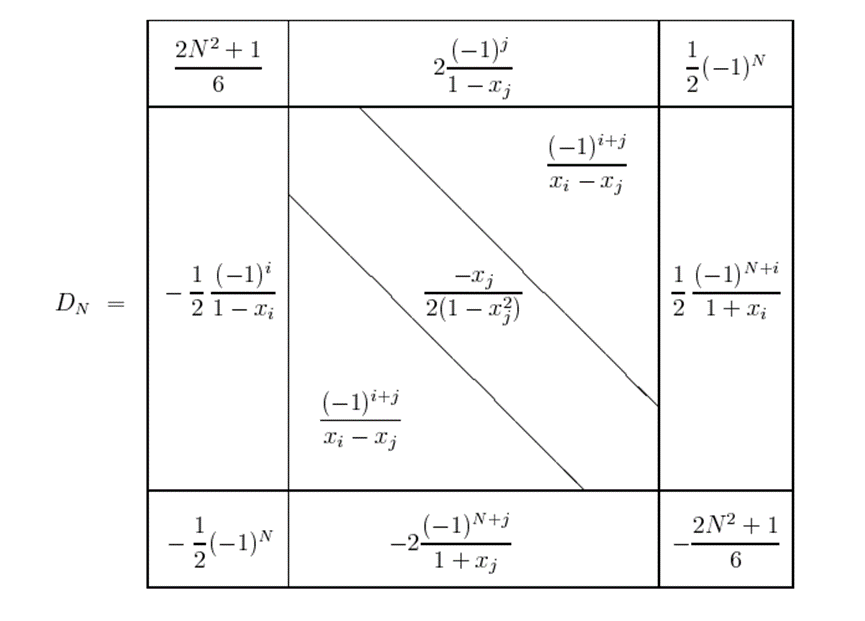
\includegraphics[width=1\textwidth]{矩阵图.png}\\
   这样我们可以用程序cheb.m 实现生成D的矩阵\\
   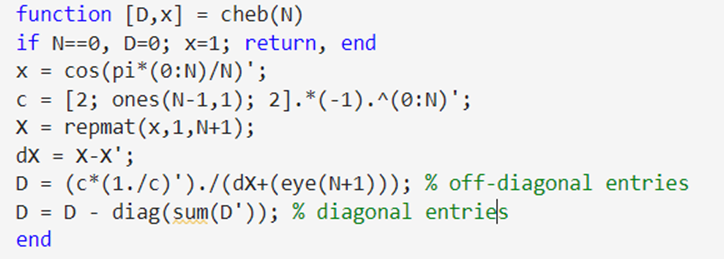
\includegraphics[width=1\textwidth]{程序图.png}\\
   我们尝试以下列程序为例体会切比雪夫配点法的精确性:\\
   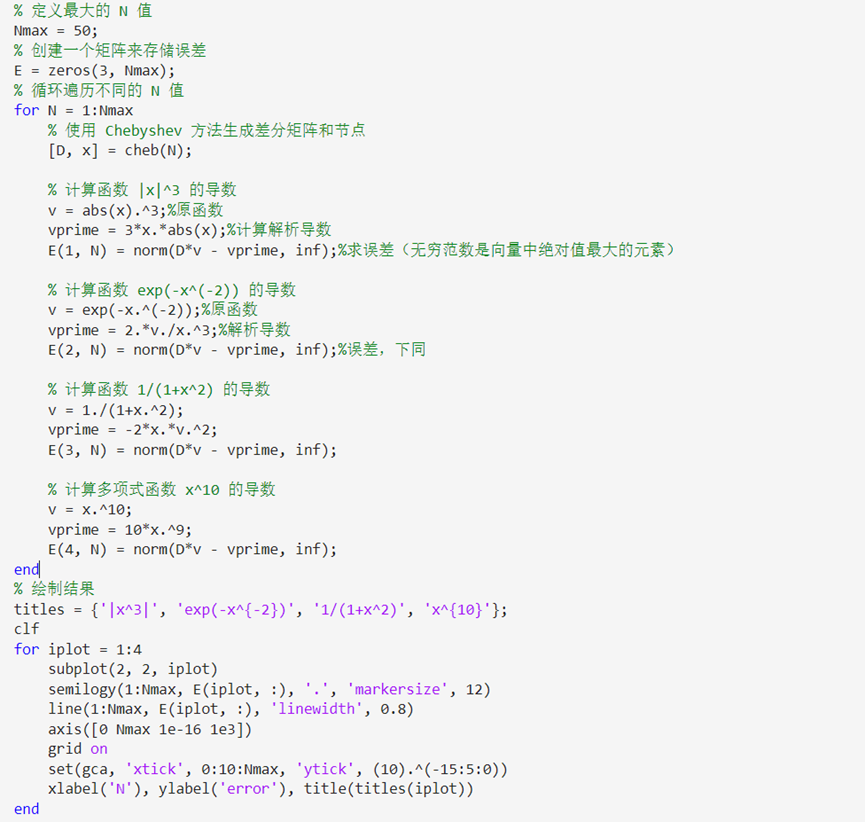
\includegraphics[width=1\textwidth]{程序图2.png}\\
   其运行结果为\\
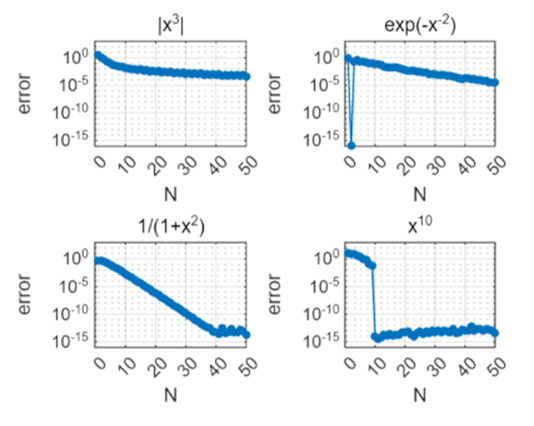
\includegraphics[width=1\textwidth]{运行结果图.png}\\
   我们可以观察到,对于性质较好的函数,我们的程序可以很快收敛到$10^-10$数量级的误差,对于性质比较“顽劣”的函数,在较高的阶数,依旧可以有不错的收敛性,切比雪夫配点法在处理比较复杂的问题上表现出很好的可用性。
   \subsection{切比雪夫配点法数值求解微分方程的思路}
   \subsubsection{线性边值问题的常微分方程:}
   \begin{equation}\label{zn9}
        u_{xx}=e^x,-1< x< 1,u(\pm)=0
   \end{equation}
   (\ref{zn9})式的解析解为:
   $$ u(x)=\frac{e^x-xsinh(4)-cosh(4)}{16}$$
  现在我们从切比雪夫配点法出发,将(\ref{zn9})式中的边界条件带入(\ref{zn8}),有$w_0=w_N=0$,故我们可以在计算该方程时去除向量的首尾两项矩阵的首位行、列,即取
  $\widetilde{D_2}=D_2(2:N,2:N)$缩减$\Vec{v}$、$\Vec{w}$首尾项,最后补上,原问题转化为$\widetilde{D^2_N}\Vec{V}=\Vec{f}$程序,对比误差\\
  以下为程序与运行结果\\
  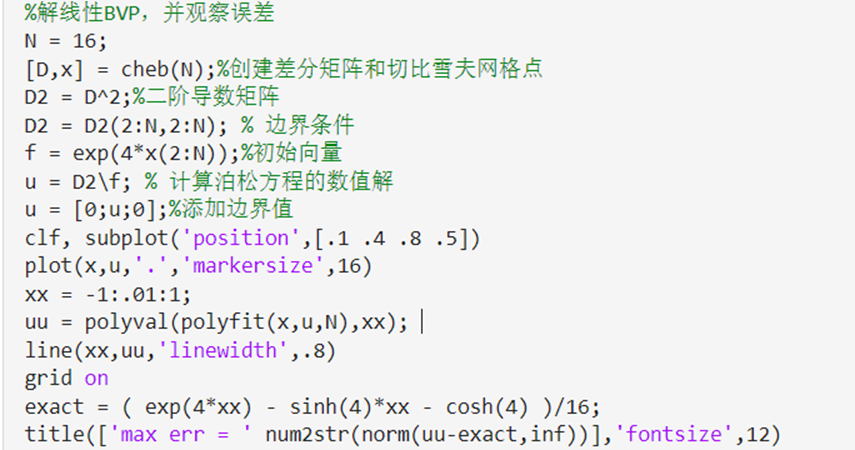
\includegraphics[width=1\textwidth]{程序图3.png}\\
   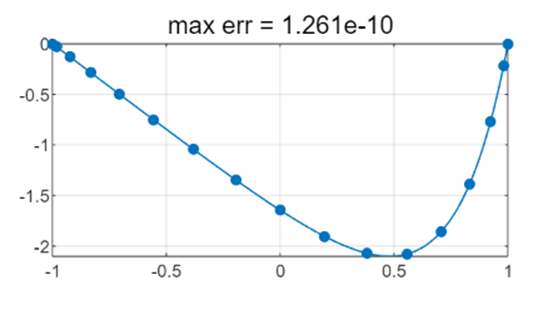
\includegraphics[width=1\textwidth]{运行结果图2.png}\\
   如图(4)可见,切比雪夫方法的收敛性良好,误差在$10^-{10}$量级。
   \subsubsection{非线性边值问题的常微分方程}
   \begin{equation}\label{zn10}
       U_{xx}=exp(u),u(\pm1)=0
   \end{equation}
   面对非线性的问题,如(\ref{zn10})式,我们无法直接列出其通用的解析式,这里可以类比不动点法,通过迭代来逼近解。即(\ref{zn10})式的方程近似为\\
   可通过迭代来逼近
   \begin{equation}\label{zn11}
\widetilde{D_N^2}\Vec{u}_{new}=exp(\Vec{v}_{old})
   \end{equation}
   以下为求解(\ref{zn11})式的程序与运行结果\\
   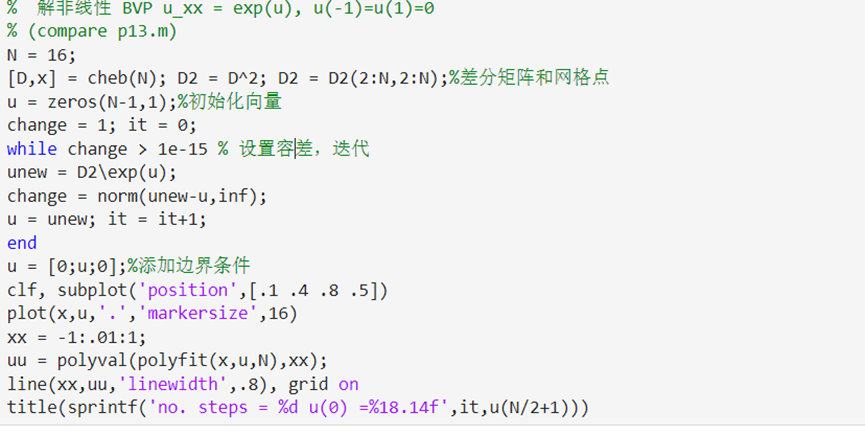
\includegraphics[width=1\textwidth]{程序图4.png}\\
   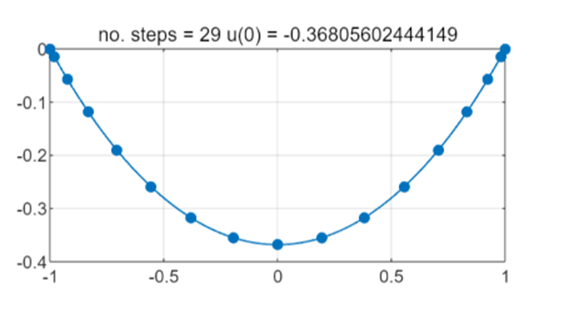
\includegraphics[width=1\textwidth]{运行结果图3.png}
   \subsubsection{泊松方程}
   泊松方程是一类在机械工程和理论物理中有着广泛应用的椭圆型偏微分方程, 经常出现在流体动力学、声学、传热学、电磁学、静电学、机械工程等诸多领域。\\
   这里我们求解一个泊松方程
   \begin{equation}\label{zn12}
   \begin{split}
       u_{xx}+u_{yy}=10sin(8x(y-1))\\
    -1<x,y<1,\text{边界u=0}
   \end{split}
   \end{equation}
   这里我们对x、y均取切比雪夫点,形成网格,并且在这些网格上取值,构成向量f。对于矩阵D,则需引入张量积的概念,其基本运算方法如下
   $$\begin{matrix}
    \text{张量积}\\
    kron(A,B)
\end{matrix}=
\begin{bmatrix}
    1&2\\
    3&4
\end{bmatrix}
\otimes 
\begin{bmatrix}
    a&b\\
    c&d
\end{bmatrix}=\begin{pmatrix}
    \begin{array}{c|c}
    \begin{array}{cc}
       a & b \\
       c & d
    \end{array} &
    \begin{array}{cc}
       2a & 2b \\
       2c & 2d
    \end{array} \\
    \hline
    \begin{array}{cc}
       3a & 3b \\
       3c & 3d
    \end{array} &
    \begin{array}{cc}
       4a & 4b \\
       4c & 4d
    \end{array}
\end{array}
\end{pmatrix}$$
这里方程的矩阵D\cite{shen2011spectral}\cite{trefethen2000spectral}需经过$L_N=I\otimes\widetilde{D}^2_N+\widetilde{D}^2_N\otimes I$的变化,该矩阵的结果往往并不十分稀疏,这可能带来运行时间和收敛精度的困扰。但好在,可以证明,在几百个维度以内,切比雪夫方法仍具有较高的精度和收敛性。将向量与矩阵对应到(\ref{zn4})式,我们得到以下程序\\
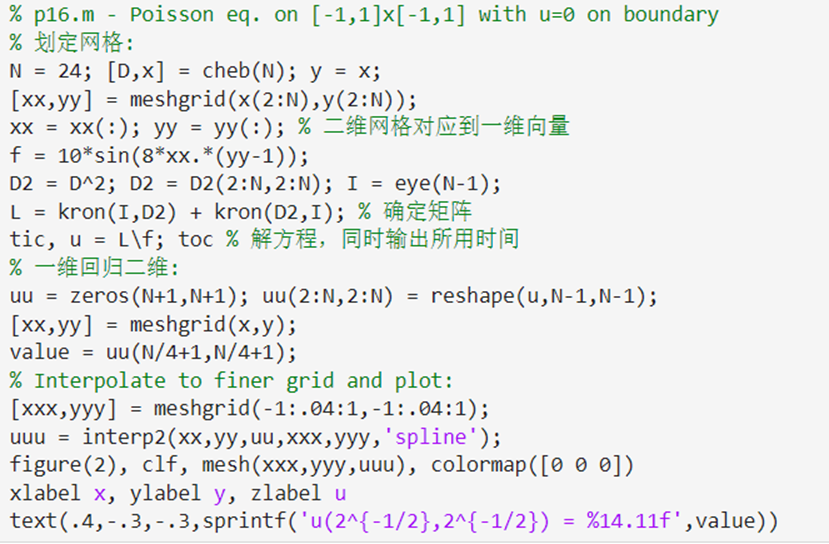
\includegraphics[width=1\textwidth]{程序图5.png}\\
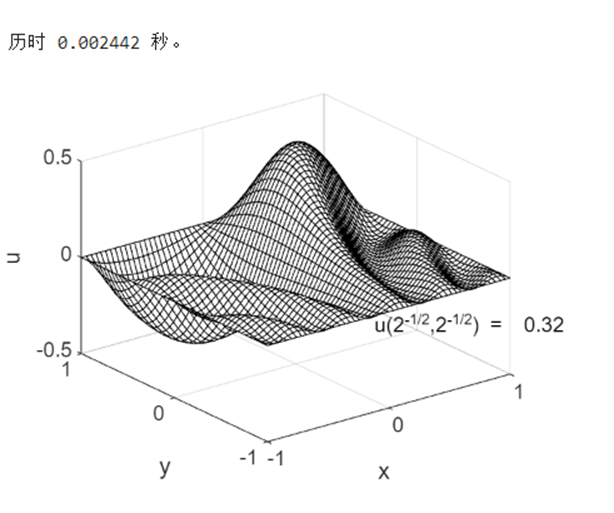
\includegraphics[width=1\textwidth]{运行结果图4.png}\\
\subsubsection{亥姆霍兹方程}
亥姆霍兹方程是一种二阶偏微分方程,用于描述波动现象的传播特性。当我们想要研究二维或三维空间中标量场的波动传播时,可以使用亥姆霍兹方程。
亥姆霍兹方程在物理学、电磁学、声学和流体力学等领域中有广泛应用
\begin{equation}\label{zn13}
\begin{split}
        \text{亥姆霍兹方程}\begin{cases}
u_{xx}+u_{yy}+k^2u=f(x,y),-1<x,y<1\\
    \text{边界处}u=0
\end{cases}\\
k=9,f(x,y)=exp(-10[(y-1)^2+(x-\frac{1}{2})^2])
\end{split}
\end{equation}
对于(\ref{zn13})所描述的问题,我们有如下程序求解。\\
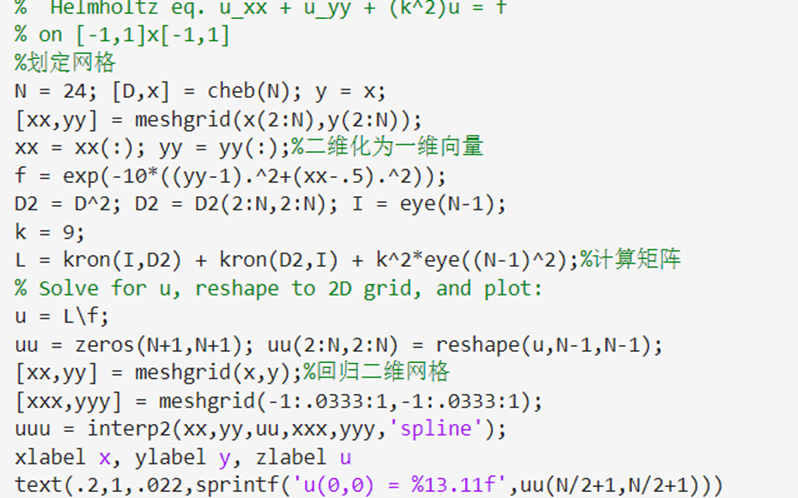
\includegraphics[width=1\textwidth]{程序图6.png}\\
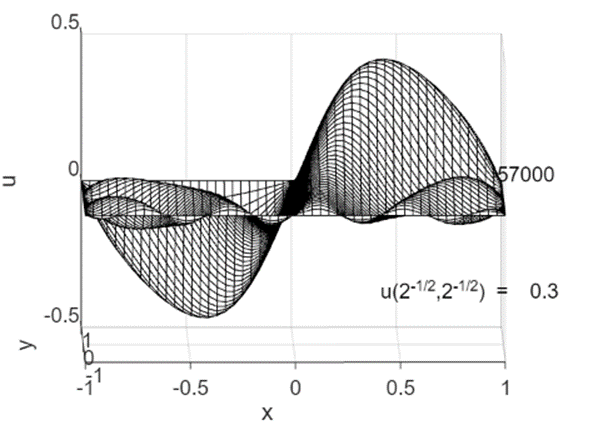
\includegraphics[width=1\textwidth]{运行结果图5.png}
































































































\section{带电粒子的电磁激发}
\subsection{引言}

在这部分中,我们将展示如何解决一维薛定谔方程,描述一个粒子置于势阱中并受到电磁脉冲激发的情况。在位置表象$|\vec{r}>$ 并以\textbf{原子单位制}中,这种情况下的方程可以表示为:
\begin{equation}
    i\dfrac{\partial\psi}{\partial t}(x,t)=\left[\dfrac{1}{2}\hat{P}^2+V(x)+A(t)\hat{P}\right]\psi(x,t)
   \label{eq:薛定谔方程}
\end{equation}

    在这里$\hat{P}$是动量算符,$A(t)$ 是磁矢势。其中$A(t)$和$V(x)$满足
    $V(x)=-V_0e^{-\alpha x^2}$ 和 
    $A(t)=A_0e^{-\frac{t^2}\sigma}\sin\omega t.$
\subsection{定态薛定谔方程}
    要解决这个方程,首先需要找到定态薛定谔方程的本征函数$\phi_n$及其对应的能量$E_n$。
    
    \begin{equation}
        \left[\dfrac{1}{2}\hat{P}^2+V(x)\right]\phi(x)=E\phi(x)
   \label{eq:定态薛定谔方程}
    \end{equation}
    
    我们将尝试一个形式的近似解:
    \begin{equation}\phi(x)=\sum_{k=0}^Na_k\varphi_k(x)
        \label{eq:定态薛定谔方程近似解}
    \end{equation}
        
式中$\varphi_k(x)=c_kH_k(x)e^{-\frac{x^2}2}$ 厄密函数

其中$H_k(x)$是 Hermite 多项式,
$c_k=\frac{1}{\sqrt{2^kk!\sqrt
\pi}}$

选择 Hermite 函数作为基函数是有道理的,因为它们是定义在实数域上的函数,且具有良好的性质,这些性质会简化我们的计算,比如以下的正交关系。
\begin{equation}
         \int_{-\infty}^{+\infty}\varphi_k(x)\varphi_{k'}(x)dx=\delta_{kk'}
\label{eq:正交性关系}
        \end{equation}

为了求得展开系数系数$a_k$,我们将近似解代入方程(\ref{eq:定态薛定谔方程})。


 \begin{equation}
    \sum_{k=0}^{N}-\frac{1}{2}\frac{d^{2}}{dx^{2}}a_{k}\varphi_{k}(x)+\sum_{k=0}^{N}V(x)\varphi_{k}(x)a_{k}=E\sum_{k=0}^{N}\varphi_{k}(x)a_{k}
\end{equation}

然后,我们将其乘以$\varphi_l(x)$并在整个实数域上进行积分。这样我们得到:
\begin{equation}
     \sum_{k=0}^{N}-\frac{1}{2}a_{k}\int_{-\infty}^{+\infty}\varphi_{l}(x)\frac{d^{2}\varphi_{k}}{dx^{2}}(x)+\sum_{k=0}^{N}a_{k}\int_{-\infty}^{+\infty}\varphi_{l}(x)V(x)\varphi_{k}(x)=E\sum_{k=0}^{N}a_{k}\int_{-\infty}^{+\infty}\varphi_{l}(x)\varphi_{k}(x)
\label{eq:定态薛定谔方程近似解}
    \end{equation}

因此,我们有3个积分要解决。由正交性关系(\ref{eq:正交性关系})直接给出了右侧积分的结果。所有我们首先处理左侧的第一个积分。

\subsubsection{第一个积分}为了解决这个积分,我们将使用以下关系式:

\begin{equation}
    \varphi^{\prime\prime}(x) = (x^2-2k-1)\varphi_k 
    \label{eq:哈哈哈}
\end{equation}
    
\begin{equation}
    x\varphi_k = \sqrt{\frac{k}{2}}\varphi_{k-1} + \sqrt{\frac{k+1}{2}}\varphi_{k+1}
    \label{eq:一次关系}
\end{equation}

通过递推关系(\ref{eq:一次关系})得:
\begin{align}
    x^{2}\varphi_{k}(x) &= x \cdot x\varphi_{k}(x) \notag \\
    &= \sqrt{\frac{k}{2}} x\varphi_{k-1}(x) + \sqrt{\frac{k+1}{2}}x\varphi_{k+1}(x) \notag \\
    &= \sqrt{\frac{k}{2}}\left(\sqrt{\frac{k-1}{2}}\varphi_{k-2}(x) + \sqrt{\frac{k}{2}}\varphi_{k}(x)\right)\notag  \\
    &\quad + \sqrt{\frac{k+1}{2}}\left(\sqrt{\frac{k+1}{2}}\varphi_{k}(x) + \sqrt{\frac{k+2}{2}}\varphi_{k+2}(x)\right)\notag \\
    &= \frac{\sqrt{k(k-1)}}{2}\varphi_{k-2}(x) + \frac{k}{2}\varphi_{k}(x) + \frac{k+1}{2}\varphi_{k}(x) + \frac{\sqrt{(k+1)(k+2)}}{2}\varphi_{k+2}(x) 
    \label{eq:二次关系}
 \end{align}
使用公式(\ref{eq:二次关系})和公式(\ref{eq:哈哈哈})的结论,我们得到,
\begin{align}
        \varphi_{k}^{\prime\prime}(x) &= \frac{\sqrt{k(k-1)}}{2}\varphi_{k-2} + \frac{2k+1}{2}\varphi_{k} + \frac{\sqrt{(k+1)(k+2)}}{2}\varphi_{k+2} - (2k+1)\varphi_{k} \\
        &= \frac{\sqrt{k(k-1)}}{2}\varphi_{k-2} + \frac{2k+1}{2}\varphi_{k} + \frac{\sqrt{(k+1)(k+2)}}{2}\varphi_{k+2}
\end{align}

即:
\begin{equation}
    \boxed{ \varphi_{k}^{\prime\prime}(x)=\frac{\sqrt{k(k-1)}}{2}\varphi_{k-2} + \frac{2k+1}{2}\varphi_{k} + \frac{\sqrt{(k+1)(k+2)}}{2}\varphi_{k+2}}
\label{eq:二阶导递推}
\end{equation}

最后,使用正交归一性关系(\ref{eq:正交性关系}),我们将第一个积分的主体部分$\int_{-\infty}^{+\infty}\varphi_{l}(x)\varphi_{k}^{\prime\prime}(x)dx$了化简为以下结果:
\begin{align}
             F_{kl} &= \int_{-\infty}^{+\infty}\varphi_{l}(x)\varphi_{k}^{\prime\prime}(x)dx \notag \\
             &= \int_{-\infty}^{+\infty}\left(\frac{\sqrt{k(k-1)}}{2}\varphi_{l}\varphi_{k-2}+\frac{2k+1}{2}\varphi_{l}\varphi_{k}+\frac{\sqrt{(k+1)(k+2)}}{2}\varphi_{l}\varphi_{k+2}\right)dx \notag \\
             &= \frac{\sqrt{k(k-1)}}{2}\delta_{k-2,l} + \frac{2k+1}{2}\delta_{kl} + \frac{\sqrt{(k+1)(k+2)}}{2}\delta_{k+2,l}
\end{align}   
即:
\begin{equation}
    \boxed{F_{kl}=\frac{\sqrt{k(k-1)}}{2}\delta_{k-2,l} + \frac{2k+1}{2}\delta_{kl} + \frac{\sqrt{(k+1)(k+2)}}{2}\delta_{k+2,l}}
\label{eq:F矩阵}
\end{equation}
\subsubsection{第二个积分}
现在,让我们来看左边的第二个积分。为了解决这个最后的积分,我们将使用高斯-勒让德(Gauss-Legendre)积分法。它允许我们将如下形式的积分表达为有限和的形式
\begin{equation}
         \int_a^bf(x)\omega(x)dy=\sum_{i=0}^N\omega_if(x_i)+K_n(f)
\label{eq:高斯-勒让德积分法}
        \end{equation}

    考虑权重函数 \( \omega(x) > 0 \) 且在区间 \([a, b]\)(有限或无限)上可积,$x_i,i=0,1,2,……N$是对应权函数生成的$n$阶正交多项式的零点,$\omega_i$取特殊的取值(具体见数值逼近的书籍)。

    由正交多项式的性质:如果 \( f \) 是一个 \( n \) 阶多项式,且其对应的阶数满足:$n<\frac{N}{2}$,(一般地,我们可以通过高阶地正交多项式保证这个条件)则 \( K_N(f) = 0 \) 。

    而对于一些一般的函数,我们可以通过取不同的 \( N \) 值来逼近这个积分,当$N$足够大时,可以近似看作$K_N(f)=0$。
    
于是,通过换元$y=\sqrt{\alpha}x$写成类如(\ref{eq:高斯-勒让德积分法})式的形式:

\begin{equation}
         \int_{-\infty}^{\infty}f(y)e^{-y^2}dy=\sum_{i=0}^{N}\omega_if(y_i)
\end{equation}

这里,\( \omega(y) = e^{-y^2} \) ,\( N> 2n \),

通过整理:
\begin{equation}
    \begin{aligned}
        & \int_{-\infty}^{+\infty}\varphi_{l}(x)V(x)\varphi_{k}(x)dx \\
        & = -V_{0}\int_{-\infty}^{+\infty}\varphi_{l}(x)e^{-\alpha x^{2}}\varphi_{k}(x)dx \\
        & = -\frac{V_{0}}{\sqrt{\alpha}}\int_{-\infty}^{+\infty}\varphi_{l}\left(\frac{y}{\sqrt{\alpha}}\right)e^{-y^{2}}\varphi_{k}\left(\frac{y}{\sqrt{\alpha}}\right)dy \\
        & = \int_{-\infty}^{+\infty}f(y)e^{-y^{2}}dy
    \end{aligned}
    \end{equation}
     

得到,$$f(y)=-\frac{V_{0}}{\sqrt{\alpha}}\varphi_{l}(\frac{y}{\sqrt{\alpha}})\varphi_{k}(\frac{y}{\sqrt{\alpha}}).$$其中当N很大时满足\( K_n(f) = 0 \)。

给定$k,l$,可在Matlab上实现高斯-勒让德积分法,

\begin{equation}
        \boxed{ U_{kl}=\int_{-\infty}^{+\infty}f(y)e^{-y^2}dy=\sum_{i=0}^{N}\omega_if(y_i)}
        \label{eq:U矩阵}
\end{equation}
     
\subsubsection{系统的矩阵形式}
我们将(\ref{eq:F矩阵})式和(\ref{eq:U矩阵})式代入(\ref{eq:定态薛定谔方程近似解})式中,得到:
\begin{equation}
    \sum_{k=0}^{N} (-\frac{1}{2}F_{kl}+U_{kl})a_k=E\delta_{kl}
\end{equation}
写成矩阵形式;
\begin{equation}
        \boxed{ \left[-\frac{1}{2}F+U\right]\vec{a}=E\vec{a}}
\end{equation}

使得系数$a_k$是向量$\vec{a}$ 的元素。这是一个特征值问题,可以用 Matlab 中的 eig 函数来求出系统中的$E_n$。
\subsection{含时的薛定谔方程}
确定了系统的本征值,我们就可以求解系统的含时演化。我们将(\ref{eq:薛定谔方程})式写为以下形式:
\begin{equation}
    i\dfrac{\partial\psi}{\partial t}(x,t)=\left[\hat{H}-iA(t)\dfrac{\partial}{\partial x}\right]\psi(x,t)=\left[E_n-iA(t)\dfrac{\partial}{\partial x}\right]\psi(x,t)
\label{eq:系统的本征方程}
\end{equation}

这里,$\hat{H}=-\frac{\partial^{2}}{\partial x^{2}}+V(x).$为系统的哈密顿算符,$E_n$为其本征值,$A(t)$为系统的外场。
     
设本征态具有形式:
\begin{align}
 \psi_n(x,t) &= b_n(t)\phi_n(x)e^{-iE_nt}
\end{align}
(这里的时间项的得出不作过多解释,等到大家学到时间演化算符就可以理解了。)
 
则一般解是这些函数的线性叠加


     \begin{equation}
    \psi_n(x,t)=\sum_{n=0}^Nb_n(t)\phi_n(x)e^{-iE_nt}
    \label{eq:本征态}
     \end{equation}

     将(\ref{eq:本征态})式代入(\ref{eq:系统的本征方程})式:
   
   得到方程的左边:
\begin{equation}
        i\frac{\partial\psi}{\partial t}(x,t) = \sum_{n=0}^{N}i b'_n(t)\phi_n(x)e^{-iE_nt} + b_n(t)\phi_n(x)E_ne^{-iE_nt} \\
       \end{equation}

    得到方程的右边:
    \begin{equation}
        \left[E_n-iA(t)\dfrac{\partial}{\partial x}\right]\psi(x,t)= \sum_{n=0}^{N}\left[E_n\phi_n(x)-iA(t)\phi'_n(x)\right]b_n(t)e^{-iE_nt}
    \end{equation}
   
    于是得到
    \begin{equation}
        \sum_{n=0}^{N}b'_n(t)\phi_n(x)e^{-iE_nt} = \sum_{n=0}^{N}-A(t)b_n(t)\phi'_n(x)e^{-iE_nt}
    \end{equation}


  在方程两边同乘以 \( \phi_m(x)e^{iE_mt} \),并在实轴上积分,以分离 \( b_{m}(t) \),从而得到$N+1$个 \( 1 \) 阶常微分方程组。因此,我们有:



  \begin{equation}  
  b_m'(t)=\sum_{n=0}^N-A(t)b_n(t)e^{-i(E_n-E_m)t}\int_{-\infty}^\infty\phi_m(x)\phi_n'(x)dx
  \label{eq:略略略}
\end{equation}  

  为了解决方程右边的积分,我们将需要以下递归关系:

\begin{equation}
        \varphi_k'(x)=\sqrt{\frac{k}{2}}\varphi_{k-1}-\sqrt{\frac{k+1}{2}}\varphi_{k+1}
    \end{equation}

利用前述关系(\ref{eq:定态薛定谔方程近似解})以及厄米特函数(Hermite functions)的正交归一性关系(\ref{eq:正交性关系}),我们得到
\begin{align}
    \int_{-\infty}^{\infty} &\left(\sum_{l=0}^{N}a_{ml}\varphi_{l}(x)\right)\left(\sum_{k=0}^{N}a_{nk}\varphi_{k}^{\prime}(x)\right)dx \notag\\
    &= \int_{-\infty}^{\infty} \left(\sum_{l=0}^{N}a_{ml}\varphi_{l}(x)\right) \left(\sum_{k=0}^{N}a_{nk}\left(\sqrt{\frac{k}{2}}\varphi_{k-1}(x)-\sqrt{\frac{k+1}{2}}\varphi_{k+1}(x)\right)\right)dx \notag\\
    &= \sum_{l=0}^{N}\sum_{k=0}^{N}a_{ml}a_{nk}\int_{-\infty}^{\infty} \left(\sqrt{\frac{k}{2}}\varphi_{l}(x)\varphi_{k-1}(x)-\sqrt{\frac{k+1}{2}}\varphi_{l}(x)\varphi_{k+1}(x)\right)dx \notag\\
    &= \sum_{l=0}^{N}\sum_{k=0}^{N}a_{ml}a_{nk}\left(\sqrt{\frac{k}{2}}\delta_{lk-1}-\sqrt{\frac{k+1}{2}}\delta_{lk+1}\right) \notag\\
    &= \sum_{k=0}^{N}a_{nk}\left(\sqrt{\frac{k}{2}}a_{m,k-1}-\sqrt{\frac{k+1}{2}}a_{m,k+1}\right)
\end{align}
    


    将结果代入上述(\ref{eq:略略略})式,得到
    \begin{equation}
       \boxed{ b'_{m}(t)=\sum_{n=0}^{N}-A(t)b_{n}(t)e^{-i(E_{n}-E_{m})t}\left[\sum_{k=0}^{N}a_{nk}\left(\sqrt{\frac{k}{2}}a_{m,k-1}-\sqrt{\frac{k+1}{2}}a_{l,k+1}\right)\right]}
    \end{equation}



    \bibliographystyle{plain}  % 选择参考文献的样式
    \bibliography{ref1}  % 指定参考文献文件的名称,不需要扩展名
\end{document}